\chapter{Simulationsumgebung}
\label{cha:simulationsumgebung}

Das Kapitel der Simulationsumgebung befasst sich mit den Eingabemöglichkeiten zur Anpassung der Simulationsparameter, sowie der konkreten Umsetzung der simulierten Welt, mit der Logik für die Notausgänge, der Personen, der Gefahrensituationen und dem Kommunikationsmodell.

Die Ausgangsbasis für die verwendeten Modelle und Protokolle stammen aus den erstellten Übungen zur Vorlesung Gensensornetze, sie wurden jedoch auf die Anforderungen der Hausarbeit adaptiert.

\section{Benutzerschnittstelle}
\label{sec:benutzerschnittstelle}


\section{Personen}
\label{sec:personen}

% Lifecycle
\subsection{Zustände}

% INIT
% INIT, DEAD
% INIT, RESCUED
% INIT, EVENT_DETECTED, DEAD
% INIT, EVENT_DETECTED, FLEEING, RESCUED
% INIT, EVENT_DETECTED, FLEEING, DEAD

\begin{figure}
\centering
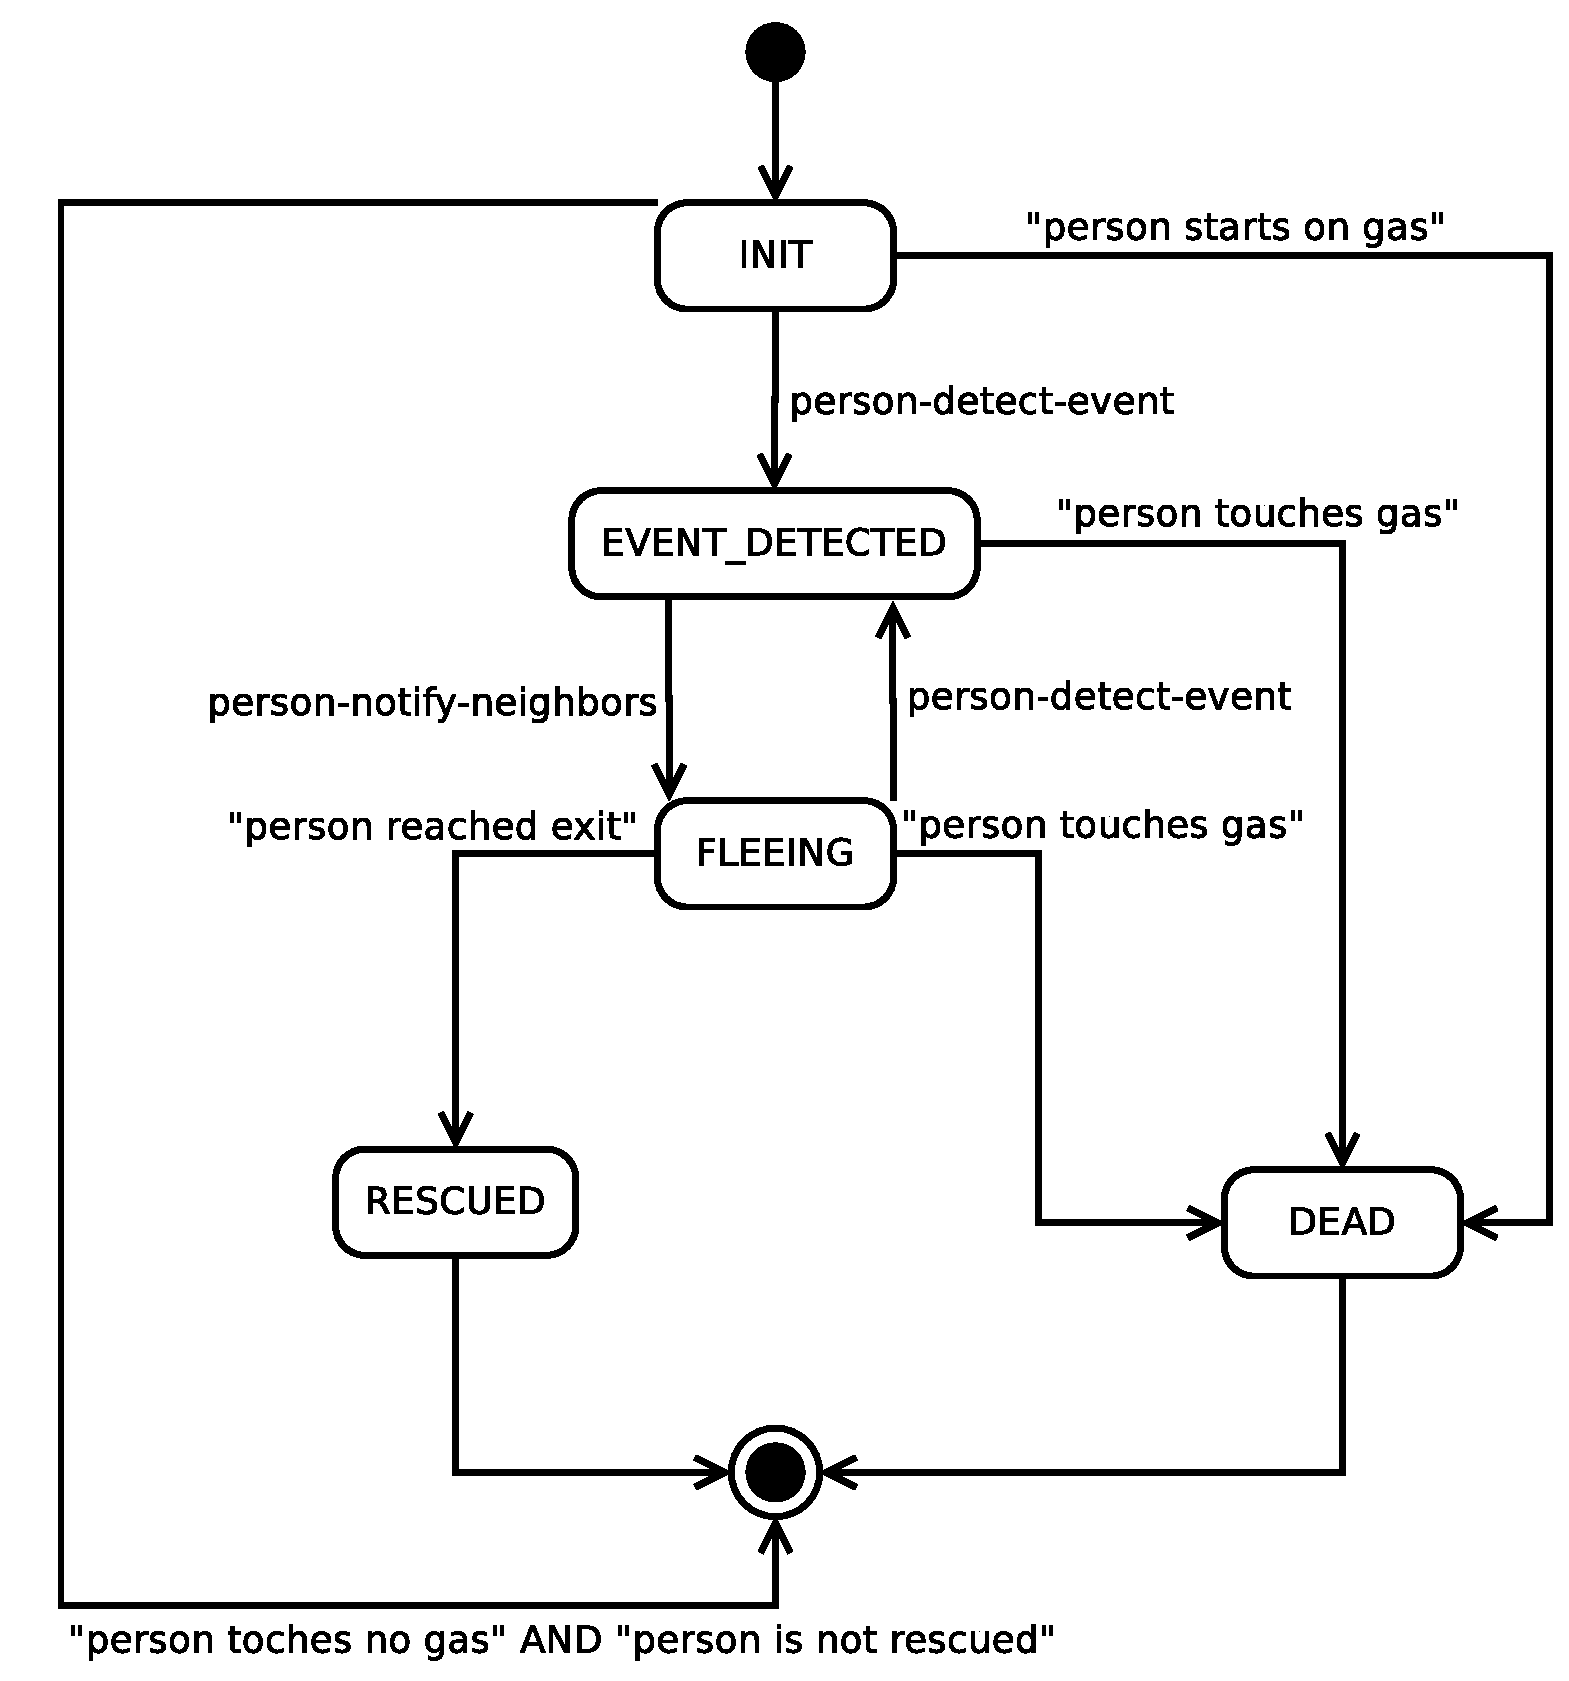
\includegraphics[height=0.6\textwidth]{simulationsumgebung/person.eps}
\caption{Zustandsdiagramm der Personen}
\label{fig:person}
\end{figure}

\subsection{Bewegungsmodell}
\label{sec:bewegungsmodell}
%Bewegungsmodell: Die Agenten sollen sich nach einem „Random Walk“ Modell bewegen. Agenten können Gefahren in ihrer Umgebung wahrnehmen und die Information an ihre nächs-ten Nachbarn weitergeben. Sobald ein Agent Informationen über eine Gefahrensituation hat, soll er sich auf dem kürzesten Weg zum nächsten Notausgang bewegen.  Hat ein Agent die Umgebung eines Notausgangs erreicht, soll er aus der Simulation genommen werden.

Dieser Abschnitt beschreibt zunächst das Bewegungsmodell der Personen ohne aktive Gefahrensituation.

\floatname{algorithm}{Algorithmus} 
\begin{algorithm}
\caption{random-walk}
\begin{algorithmic} 
\STATE nb $\leftarrow$ one-of neighbors
\WHILE{\textit{[patch-state] of nb = WALL}}
\STATE nb $\leftarrow$ one-of neighbors 
\ENDWHILE
\STATE face nb
\STATE forward 1
\end{algorithmic}
\end{algorithm}


\subsection{Kommunikationsmodell}
\label{sec:kommunikationsmodell}
%Kommunikationsmodell: Als Kommunikationsmodell können beliebige Modelle der Vorlesung implementiert werden. Dabei sollte insbesondere auf die dynamische Netzwerktopologie geach-tet werden. 

\floatname{algorithm}{Protokoll} 
\begin{algorithm}
\caption{Warnung vor Gefahrensituationen}
\begin{algorithmic} 
\STATE \textit{State Trans. Sys.:} $\langle\{$INIT, EVENT{\_}DETECTED, FLEEING, RESCUED, DEAD$\}\rangle$
\STATE \textit{Initialization:} All notes in state INIT
\STATE \textit{Restrictions:} Reliable communication; connected, bidirected communication graph $G = (V,E)$, neighborhoodfunction nbr: $V \rightarrow 2^{V}$
\STATE \textit{Local data:}

\STATE $ $
\STATE \textbf{INIT}
\STATE Receiving(\textit{event{\_}detected})
\WHILE{\textit{not event{\_}detected}}
\STATE random-walk
\STATE create-graph($G$)\hfill\emph{; generate complete new graph}
\ENDWHILE
\STATE become EVENT{\_}DETECTED


\STATE $ $
\STATE \textbf{EVENT{\_}DETECTED}
\STATE broadcast(\textit{event{\_}detected})\hfill\emph{; broadcast event detection to linked neighbors}
\STATE become FLEEING

\STATE $ $
\STATE \textbf{FLEEING}
\STATE broadcast(\textit{event{\_}detected})\hfill\emph{; rebroadcast event detection to linked neighbors}
\WHILE{\textit{not person-reach-exit}}
\STATE person-move-to-exit\hfill\emph{; using orientation-algorithm}
\STATE create-graph($G$)\hfill\emph{; generate complete new graph}
\IF{touching-gas}
\STATE become DEAD
\ENDIF
\ENDWHILE
\STATE become RESCUED

\STATE $ $
\STATE \textbf{RESCUED}
\STATE create-graph($G$)\hfill\emph{; generate complete new graph without note}

\STATE $ $
\STATE \textbf{DEAD}
\STATE create-graph($G$)\hfill\emph{; generate complete new graph without note}

\end{algorithmic}
\end{algorithm}

\section{Notausgänge}
\label{sec:notausgaenge}
%Notausgänge: Notausgänge sollen als statische Sensorknoten modelliert werden, die ihre Po-sition sowie Information zu ihrer Passierbarkeit im Netz verteilen. Die Positionen dieser sog. anchor nodes sollen zur Positionierung der mobilen Sensorknoten verwendet werden (Algorithmik). Während einer Simulation sollte der Ausfall einzelner Notausgänge simuliert werden.

%Lifecycle
\subsection{Zustände}

% INIT, NEGOTIABLE
% INIT, NEGOTIABLE, BLOCKED

\begin{figure}
\centering
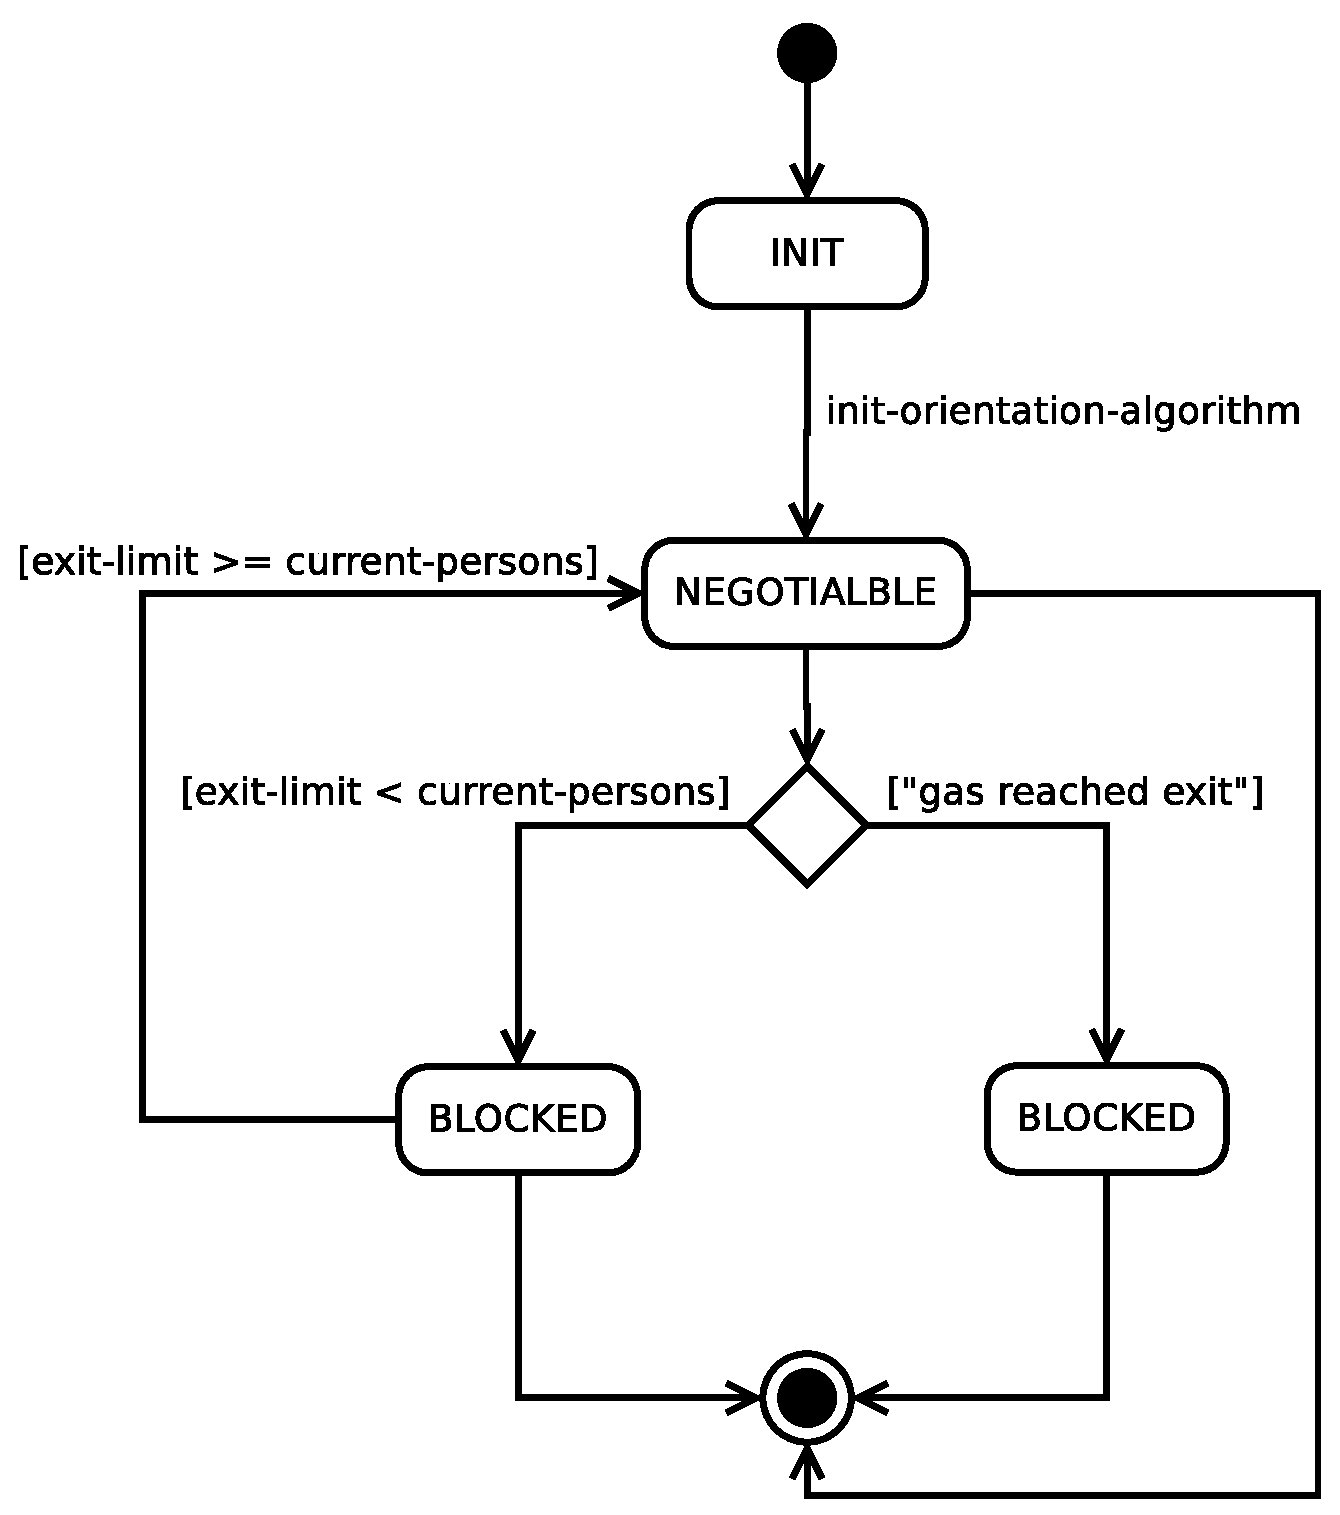
\includegraphics[height=0.6\textwidth]{simulationsumgebung/exit.eps}
\caption{Zustandsdiagramm der Notausgänge}
\label{fig:exit}
\end{figure}

%\begin{algorithm}
%\caption{Patch-Flooding (Zellulärer Automat)}
%\begin{algorithmic} 
%\STATE \textit{State Trans. Sys.:} $\langle\{$NONE$\},\{$NONE, SPREADING, IDLE, DONE$\}\rangle$
%\STATE \textit{Initialization:} All patches in state NONE
%\STATE \textit{Restrictions:} orientation-algorithm = $"$Cellular automaton$"$
%\STATE \textit{Global data:} exit-signal-strength $\in \mathbb{N}_{\geq0}$
%\STATE \textit{Local data:} 
%\STATE Set \textit{exits} of exits in range
%\STATE Set \textit{signal-noises} of exit signals
%
%\STATE $ $
%\STATE \textbf{NONE}
%\STATE \textit{Spontaneously}
%\STATE exits $\leftarrow$ myself\hfill\emph{;exit on this patch}
%\STATE signal-noises $\leftarrow$ 0
%\STATE become SPREADING
%
%
%\STATE $ $
%\STATE \textbf{SPREADING}
%\STATE parent-exit $\leftarrow$ exit
%\STATE signal-noise-here $\leftarrow$ signal-noise + 1
%\FOR{? one-of neighbors}
%\IF{[patch-state] of ? = NONE}
%\STATE exits $\leftarrow$ parent-exit
%\STATE signal-noises $\leftarrow$ signal-noise-here
%\ENDIF
%\ENDFOR
%\STATE become IDLE
%
%
%\STATE $ $
%\STATE \textbf{IDLE}
%
%\STATE become DONE
%
%\STATE $ $
%\STATE \textbf{DONE}
%
%\end{algorithmic}
%\end{algorithm}


\section{Gefahrensituationen}
\label{sec:gefahrensituationen}
%Gefahrenevents: Gefahrenevents erscheinen an zufälligen Orten im Grundriss. Ihr Erscheinen sollte zur vollständigen Evakuierung des Areals führen.

%Lifecyle
\subsection{Zustände}

% INIT, COUNTDOWN, GASSING, DONE

\begin{figure}
\centering
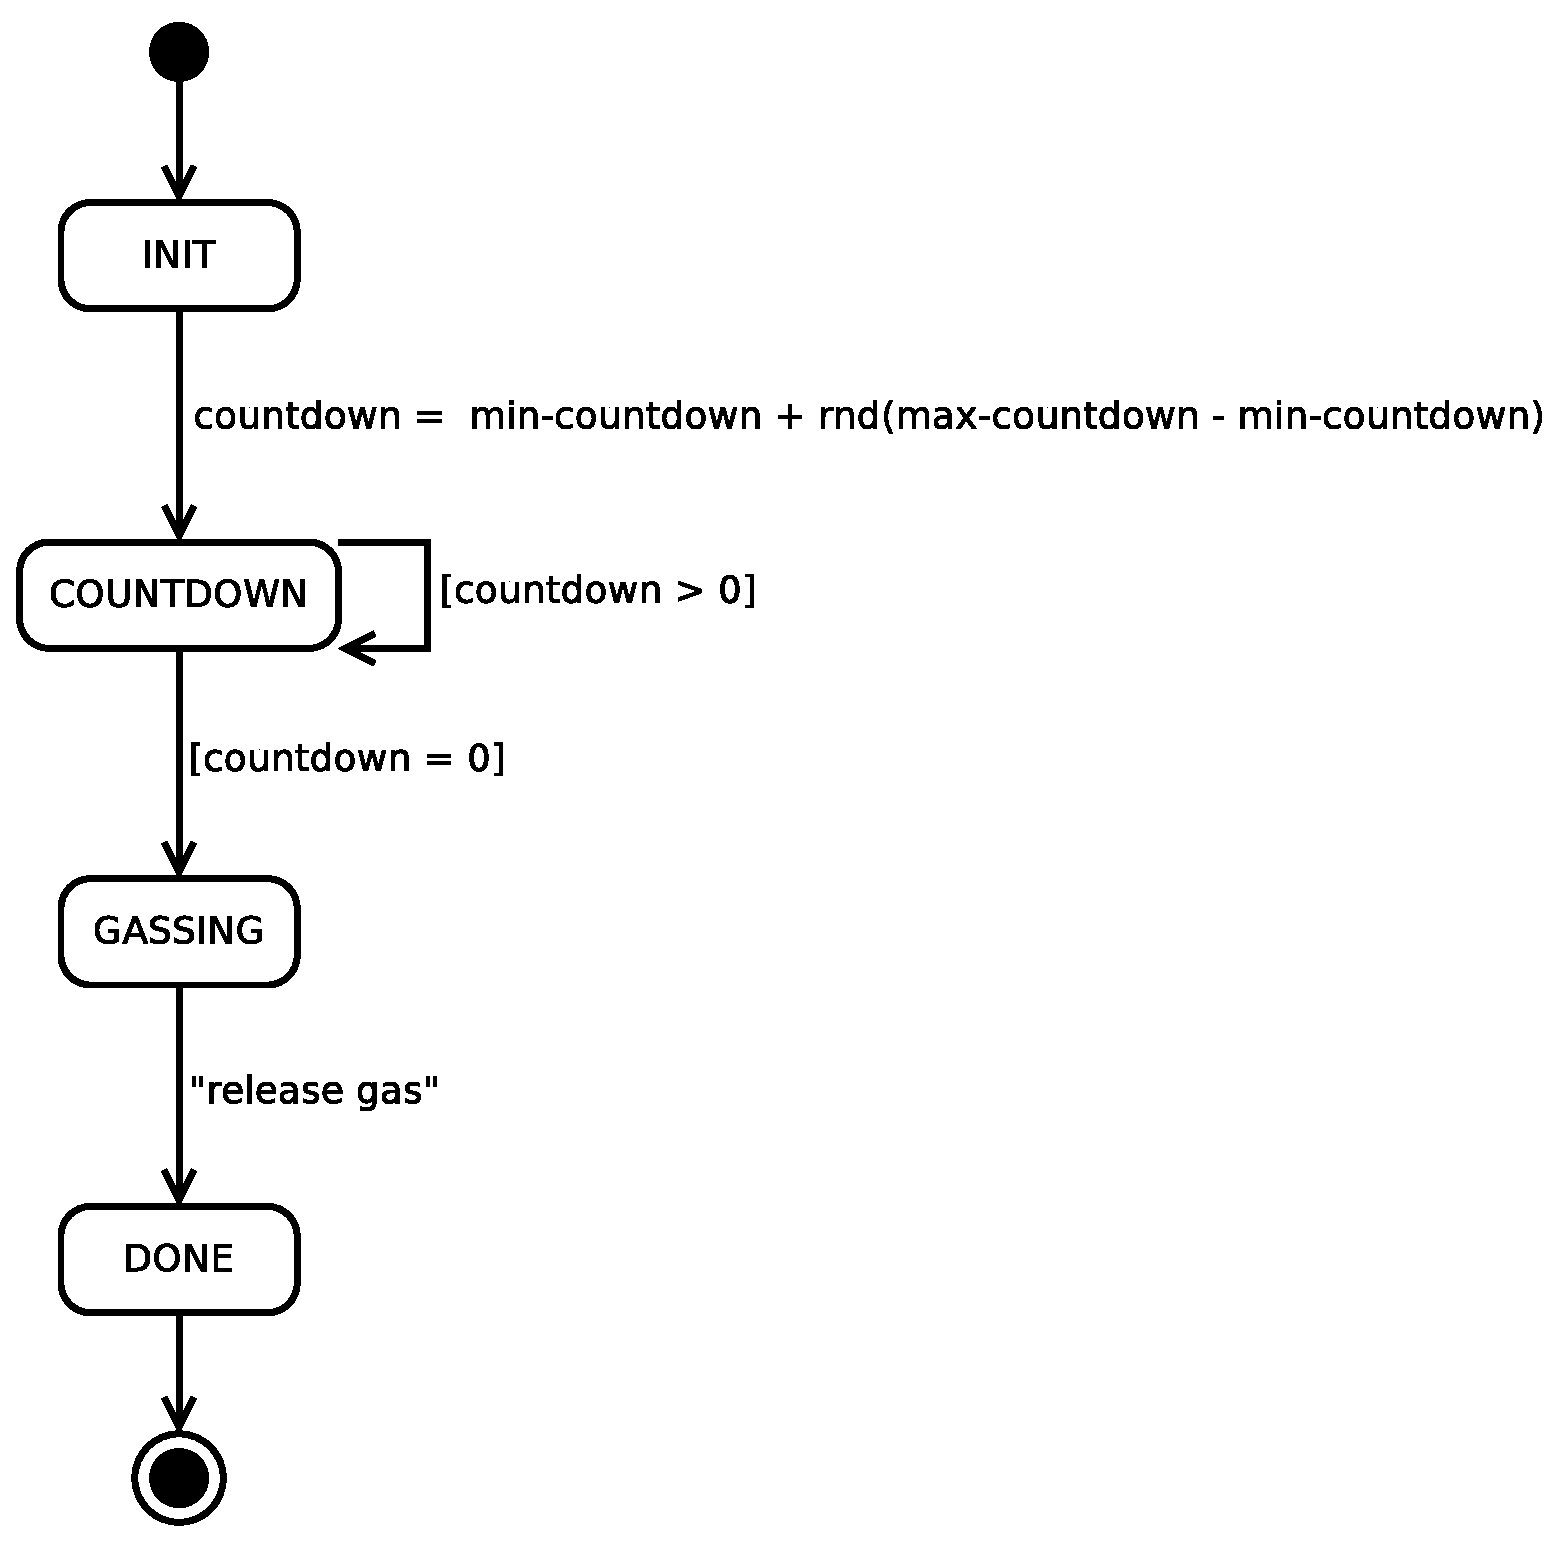
\includegraphics[height=0.6\textwidth]{simulationsumgebung/event.eps}
\caption{Zustandsdiagramm der Gefahrenevents}
\label{fig:event}
\end{figure}

\floatname{algorithm}{Protokoll} 
\begin{algorithm}
\caption{Gefahrensituation}
\begin{algorithmic} 
\STATE \textit{State Trans. Sys.:} $\langle\{$INIT, COUNTDOWN, GASSING, DONE$\}\rangle$
\STATE \textit{Initialization:} All notes in state INIT
\STATE \textit{Restrictions:} All patches in state $\{$NONE, DONE$\}$
\STATE \textit{Local data:} countdown $\in \mathbb{N}_{\geq0}$ 
\STATE $ $
\STATE \textbf{INIT}
\STATE \textit{Spontaneously}

\STATE countdown $\leftarrow$ minCountdown + (random (maxCountdown - minCountdown))
\STATE become COUNTDOWN


\STATE $ $
\STATE \textbf{COUNTDOWN}
\STATE countdown $\leftarrow$ countdown - 1
\IF{$countdown = 0$}
\STATE become GASSING
\ENDIF

\STATE $ $
\STATE \textbf{GASSING}
\STATE ask patch-here $[$ patch-state $\leftarrow$ EVENT $]$ 
\STATE become DONE

\STATE $ $
\STATE \textbf{DONE}

\end{algorithmic}
\end{algorithm}


\section{Patches}
\label{sec:patches}

%Lifecyle
\subsection{Implizite Zustände}

% NONE, WALL, SPREADING, IDLE, DONE, EVENT, EVENT-DONE

% Kategorie: Grundriss
% NONE
% WALL

% Kategorie: Zellulärer Automat
% NONE
% NONE, SPREADING, IDLE, DONE

% Kategorie: Gefahrensituation
% NONE, EVENT
% NONE, EVENT, EVENT_DONE
% DONE, EVENT
% DONE, EVENT, EVENT_DONE

\begin{figure}
\centering
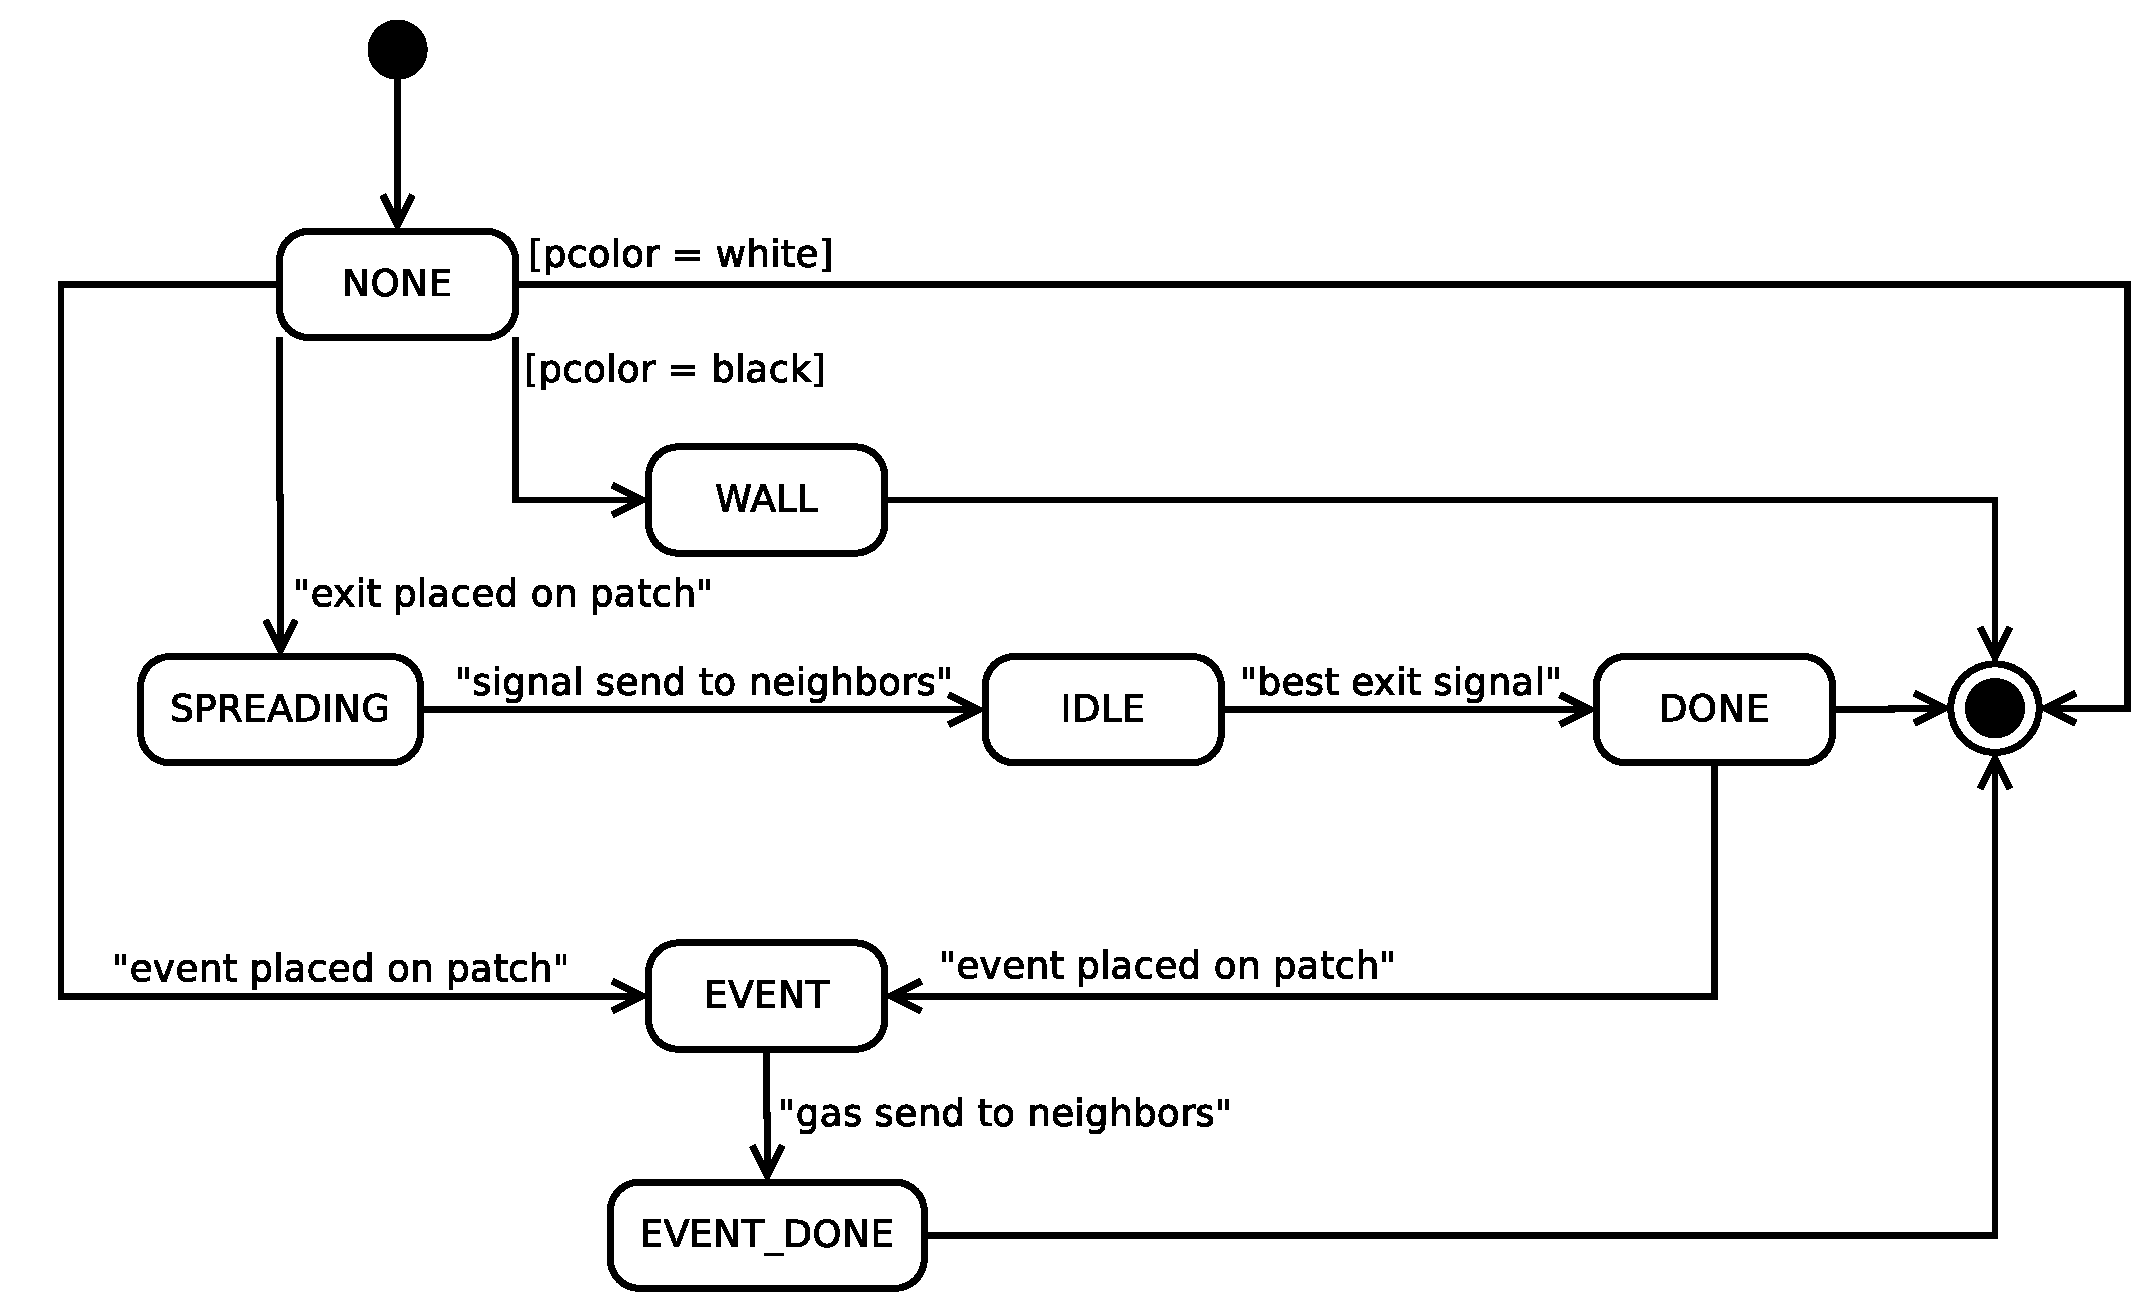
\includegraphics[height=0.6\textwidth]{simulationsumgebung/patch.eps}
\caption{Zustandsdiagramm der Patches}
\label{fig:patch}
\end{figure}

\section{Ressourcen der Simulationsumgebung}
\label{sec:ressourcen}

Die Simulationsumgebung wird über die Datei \verb|Evakuierung.nlogo| gestartet. Der Programmcode ist nach Funktion und \emph{Breed}-Klasse unterteilt.

\paragraph{Gefahrensituationen} 

\begin{verbatim}
event.nls
event-gassing.nls
\end{verbatim}

Die Quellcode-Datei \verb|event.nls| beinhaltet den Lebenszyklus der Gefahrenevents und deren Zustandsübergangsprotokoll. Mittels \verb|event-gassing.nls| wird die Ausbreitung des Giftgases implementiert, die größtenteils den Patch-Lebenszyklus manipuliert.

\paragraph{Lokalisierung}

\begin{verbatim}
locate.nls
\end{verbatim}

In dieser Datei wird der Algorithmus zur Lokalisierung aus dem Paper \cite{Jonathan.2004} implementiert.

\paragraph{Notausgänge}

\begin{verbatim}
exit.nls
exit-cellular-automaton.nls
exit-gsn.nls
\end{verbatim}

Die Quellcode-Datei \verb|event.nls| steuert den Setup und den Lebenszyklus der Notausgänge. Mittels \verb|exit-cellular-automaton.nls| wird der Orientierungsalgorithmus auf Basis des zellulären Automats realisiert. Letztlich definiert die Datei \verb|exit-gsn.nls| das Kommunikationsmodell zur Übermittlung der Statusinformationen.

\paragraph{Personen}

\begin{verbatim}
person.nls
person-gsn.nls
person-linking.nls
\end{verbatim}

\verb|person.nls| regelt den Setup der Personen und deren Lebenszyklus. \verb|person-gsn.nls| umfasst den Quellcode für die Kommunikation zwischen Personen und mit der Datei \verb|person-linking.nls| wird der Graph zwischen Personen erstellt.

\paragraph{Simulationswelt}

\begin{verbatim}
patch.nls
\end{verbatim}

Hier wird der Quellcode für den Lebenszyklus der \emph{Patches} definiert.